\documentclass[
    11pt,
    a4paper,
    sfdefaults=false,
    toc=chapterentrywithdots,
    twoside,openright,
    titlepage,
    parskip=half,
    headings=normal,  % reduces heading size
    listof=totoc,
    bibliography=totoc,
    index=totoc,
    captions=tableheading,  % caption below table
    chapterprefix,
    listof=flat,
    final
]{scrbook}


% details about your thesis
\newcommand{\titel}{Gefahren im Metaverse: Social Engineering als Grundlage für Angriffe im Metaverse}
\newcommand{\artderarbeit}{Bachelorarbeit}  % {Bachelorarbeit,Masterarbeit}
\newcommand{\autor}{Andre Schindler}
\newcommand{\studiengang}{Wirtschaftsinformatik}  % {Informatik,Wirtschaftsinformatik,Medieninformatik}
\newcommand{\matrikelnr}{327\,2457}
\newcommand{\erstgutachter}{Prof.\,Dr.~Ronald Petrlic}
\newcommand{\zweitgutachter}{Prof.\,Dr.~Peter Rausch}
\newcommand{\betreuer}{M.Sc.\,~Martina Schmidt}
\newcommand{\unternehmen}{Musterfirma GmbH}
\newcommand{\logo}{figures/TH-Nuernberg-RGB.png}
\newcommand{\keywords}{hot, fuzz}
 

% custom head and foot
\usepackage[automark]{scrlayer-scrpage}
\pagestyle{scrheadings}
\ihead{\headmark}
\chead{}
\ohead{\pagemark}
\renewcommand*\chaptermarkformat{\chapappifchapterprefix{\ }% 
  \thechapter.\enskip}

\RedeclareSectionCommand[tocindent=10pt]{section}
\RedeclareSectionCommand[tocindent=18pt]{subsection}
%\RedeclareSectionCommand[tocnumwidth=0pt]{chapter}

\usepackage{scrhack}

% other packages
\usepackage[utf8]{inputenc}
\usepackage[T1]{fontenc}
\usepackage{lmodern,relsize,textcomp,csquotes}
\usepackage{amsmath,amsfonts}
\usepackage[ngerman]{babel}  % flip for German thesis
\usepackage[final]{graphicx}
\usepackage{setspace,geometry,xcolor}
\usepackage{makeidx}
\usepackage{paralist,ifthen,todonotes}
\usepackage{url}
\usepackage[toc, style=alttree]{glossaries}
\usepackage{pdfpages}

% table setup
\usepackage{longtable}
\usepackage{array}
\usepackage{ragged2e}
\usepackage{lscape}

% pdf hyperref
\usepackage[
    bookmarks=true,
    bookmarksopen=true,
    bookmarksnumbered=true,
    bookmarksopenlevel=1,
    pdftitle={\titel},
    pdfauthor={\autor},
    pdfcreator={\autor},
    pdfsubject={\titel},
    pdfkeywords={\keywords},
    pdfpagelabels=true,
    colorlinks=true,
    linkcolor=red,
    urlcolor=magenta,
    anchorcolor=black,
    citecolor=cyan,
    filecolor=magenta,
    menucolor=red,
    plainpages=false,
    hypertexnames=true,
    linktocpage=true,
]{hyperref}

% configure your listings style
\usepackage{listings}
\lstset{
	tabsize=3,
	extendedchars=true,
	frame=single,
	showstringspaces=true,
	numbers=left,
	numberstyle=\small,
	breakautoindent=true
}

% page setup
% \setlength{\topskip}{\ht\strutbox}
\geometry{paper=a4paper,left=2.5cm,top=3.0cm,bindingoffset=.8cm}
\onehalfspacing
\frenchspacing
\clubpenalty = 10000
\widowpenalty = 10000 
\displaywidowpenalty = 10000

% some commands
\newcommand{\ua}{\mbox{u.\,a.\ }}
\newcommand{\zB}{\mbox{z.\,B.\ }}
\newcommand{\dahe}{\mbox{d.\,h.,\ }}
\newcommand{\bzw}{\mbox{bzw.\ }}
\newcommand{\bzgl}{\mbox{bzgl.\ }}
\newcommand{\eg}{\mbox{e.\,g.\ }}
\newcommand{\ie}{\mbox{i.\,e.\ }}
\newcommand{\wrt}{\mbox{w.\,r.\,t.\ }}
\newcommand{\etal}{\mbox{\emph{et.\,al.\ }}}


% TODO remove if not needed...
\usepackage{blindtext}

% load glossary entries
\makenoidxglossaries
\loadglsentries{glossary}
\glssetwidest{Immersion} %Glossar spaltenbreite festlegen

\begin{document}

\setcounter{secnumdepth}{3}  % numerate subsections
\setcounter{tocdepth}{2}  % ...but don't include them in toc

\frontmatter
\include{cover}\cleardoublepage

% download the following form and complete it (hit save in your editor)
% https://intern.ohmportal.de/fileadmin/Gelenkte_Doks/Abt/SZS/SB/SB_0050_FO_Pruefungsrechtliche_Erklaerung_und_Erklaerung_zur_Veroeffentlichung_der_Abschlussarbeit_public.pdf
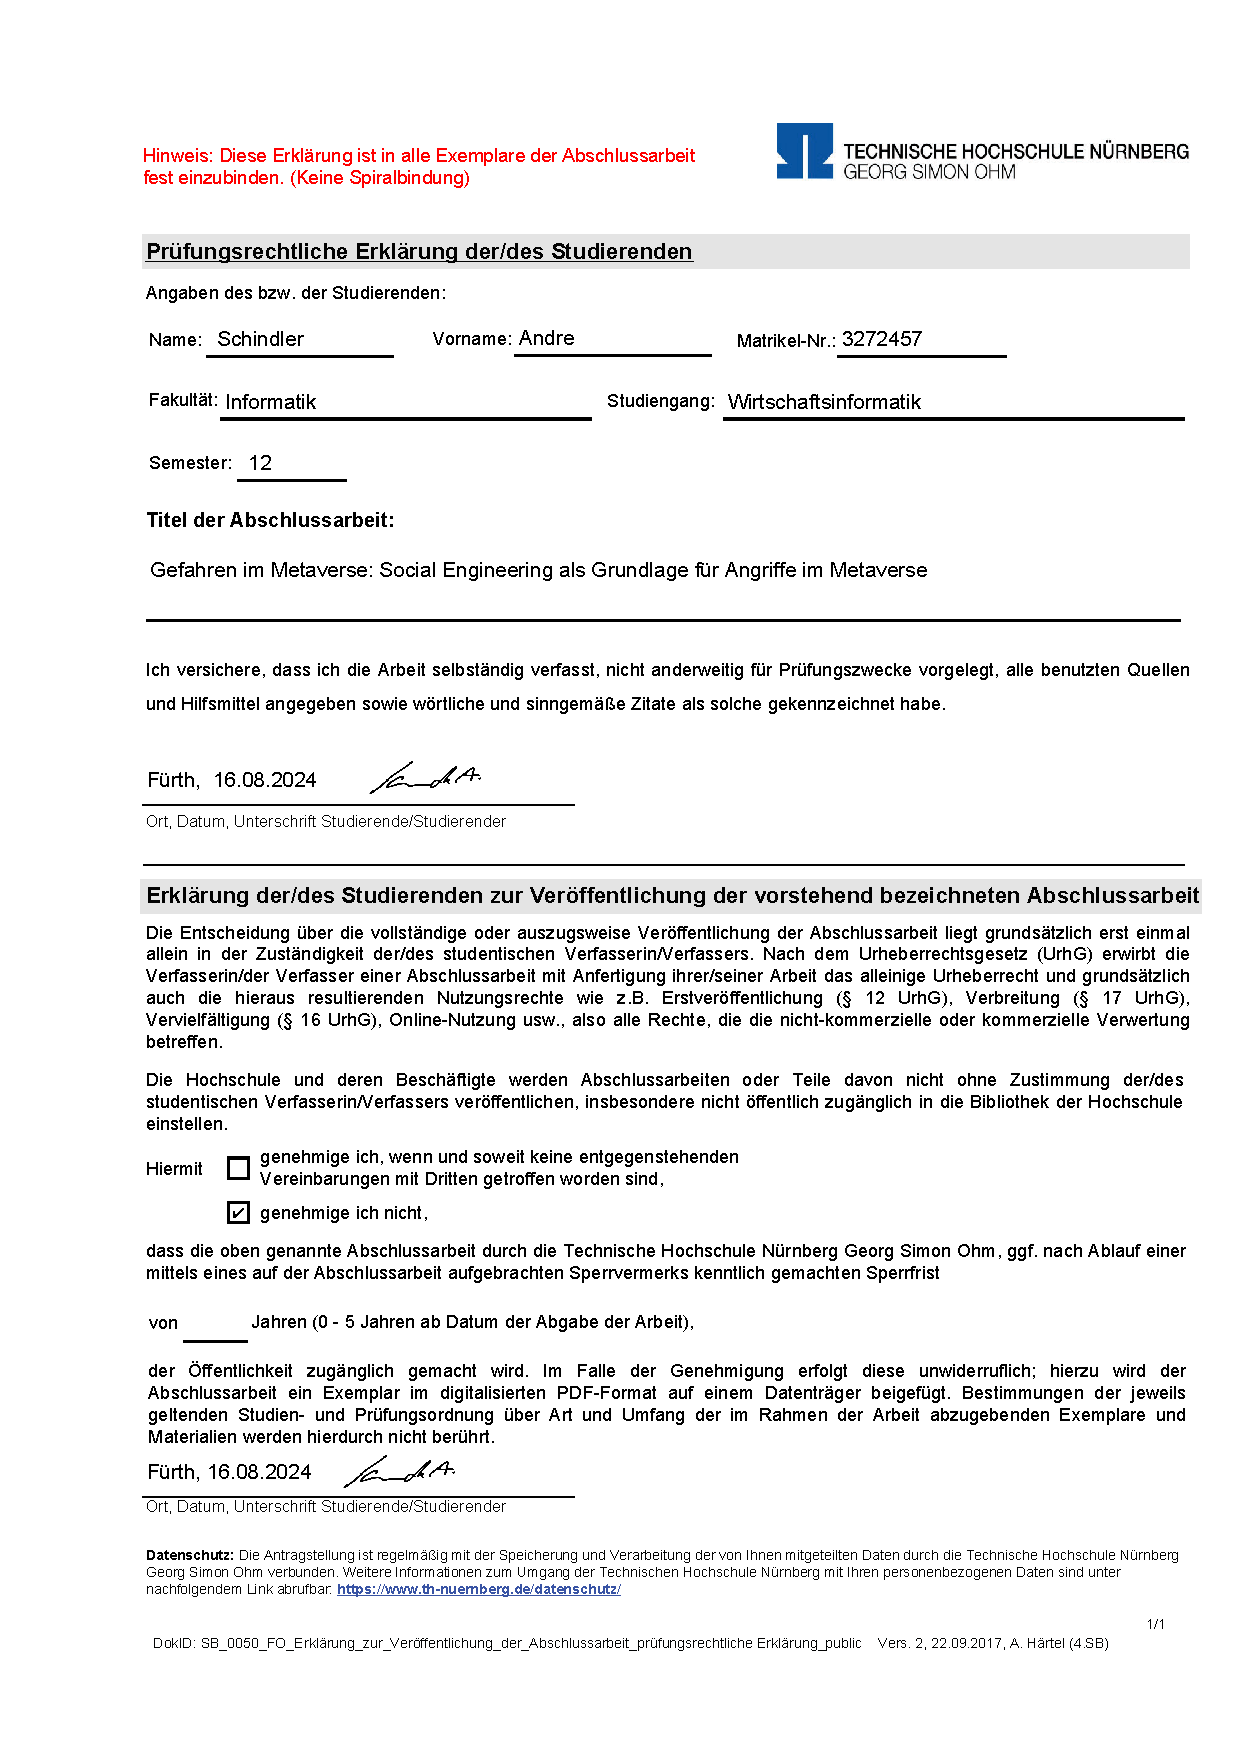
\includepdf{SB_0050_FO_Pruefungsrechtliche_Erklaerung_und_Erklaerung_zur_Veroeffentlichung_der_Abschlussarbeit_public.pdf}\cleardoublepage

%\chapter{Anleitungen und Tests}\label{ch:Anleitungen}

\section{Anleitungen}

\paragraph*{Glossar}

Glossar erstellen \url{https://www.lektorat-bachelorarbeit.de/glossar-erstellen/#:~:text=In%20einem%20Glossar%20sammelt%20man,die%20Erstellung%2C%20beantwortet%20dieser%20Text.} \\
It is possible to reference glossary entries as \gls{library} as an example.

\paragraph{Bilder einfügen}
nach paragraph muss was stehen bevor das bild kommt

\begin{figure}[!h]
    \centering
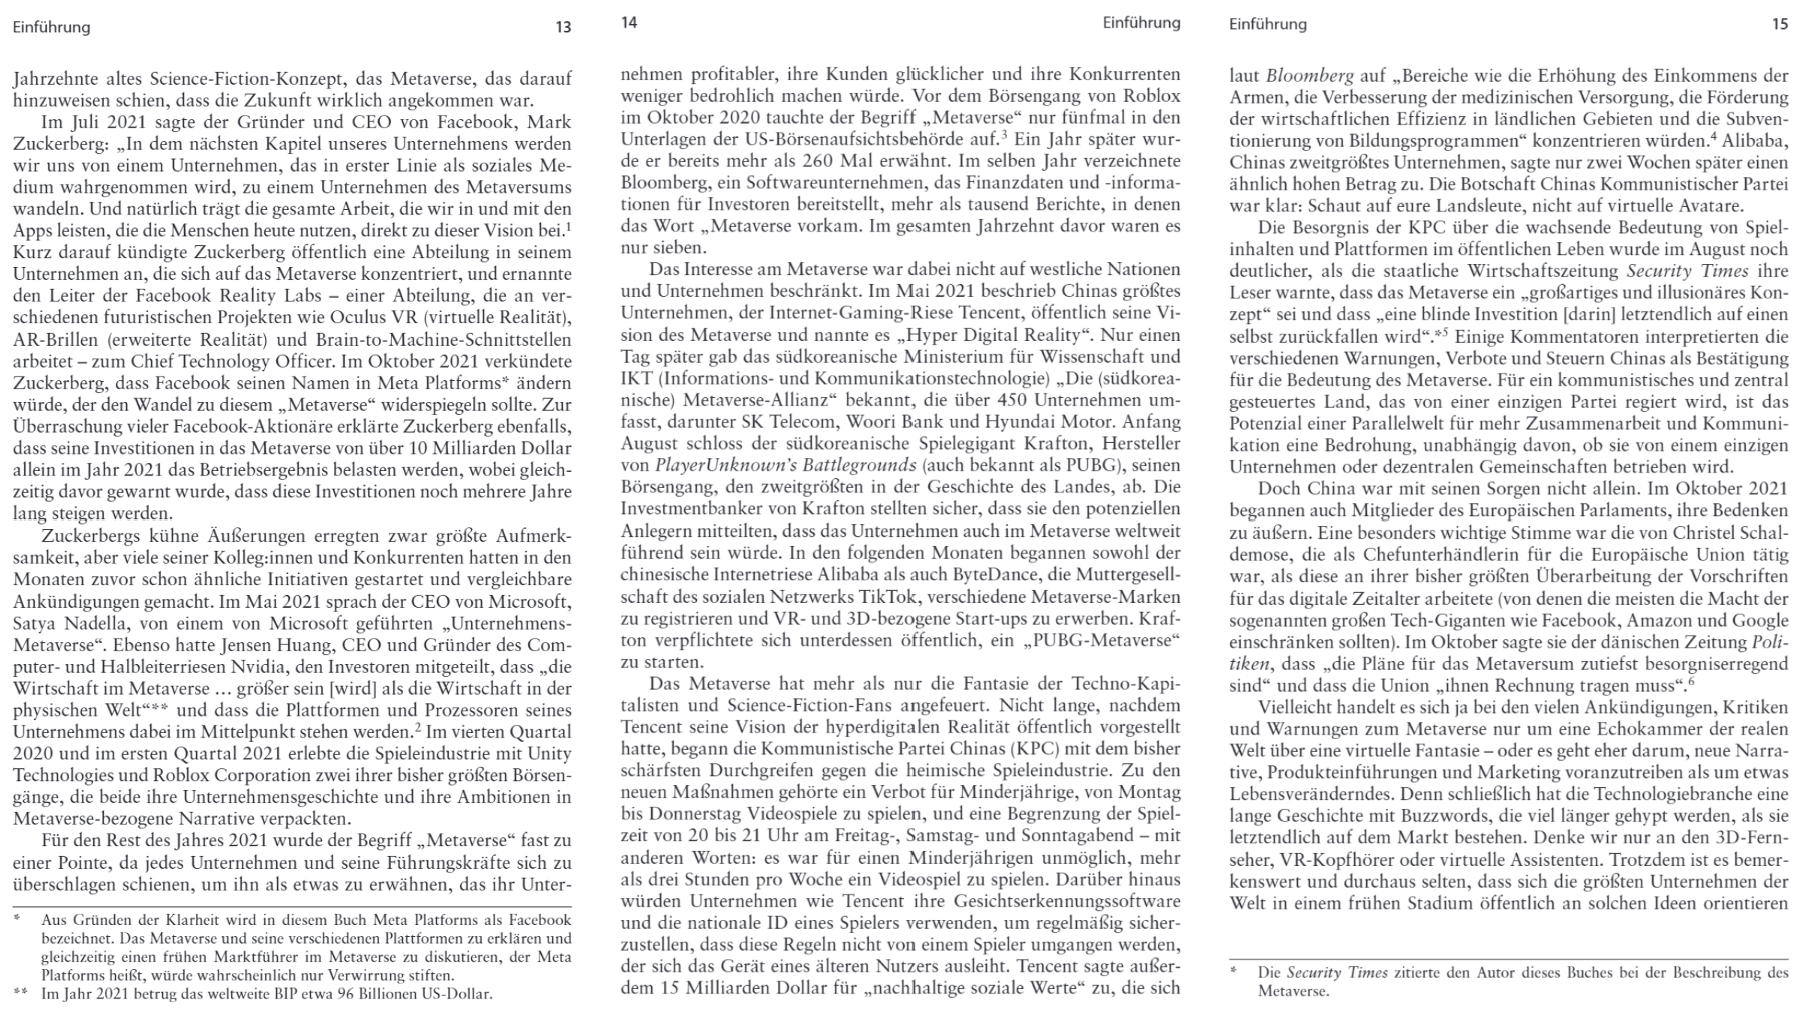
\includegraphics[width = 15cm]{figures/Das_Metaverse_uwearw13-15.png}
\caption{Das Metaverse und wie es alles revolutionieren wird}
\cite{Ball22}
\label{fig:testbild}
\end{figure}

%In this chapter, we're actually using some code!\\

%\begin{lstlisting}[language=Python,caption={This is an example of inline listing},captionpos=b]
%x = 1
%if x == 1:
%    # indented four spaces
%    print("x is 1.")

%\end{lstlisting}

%You can also include listings from a file directly:

%\lstinputlisting[language=Python,caption={This is an example of included listing},captionpos=b]{listings/example.py}


\section*{Tests}

Definitionen Metaverse \cite{Ball22}
\\Definitionen Metaverse \cite{Ball22a}
\\Definitionen Metaverse \cite{Drip22} \\
Seite 46 gegen wen Kämpfen wir \cite{Hypp22}\\
Psychologie hinter SocialEngeneering \cite{schu11}\\
\\

URL einfügen \url{https://ar5iv.labs.arxiv.org/html/2401.05569}


You can also write footnotes.\footnote{Footnotes will be positioned automatically.}

äüö

\include{content/0_abstract}\cleardoublepage

\tableofcontents

\mainmatter
\chapter{Einleitung}\label{ch:Einleitung}

Das Metaverse, ein umfassender virtueller Raum, der durch die Kombination physischer und virtueller Realität entsteht, hat in den letzten Jahren erhebliche Aufmerksamkeit auf sich gezogen. Es wird als die nächste große Entwicklung des Internets angesehen, die eine völlig neue Dimension der Interaktion und des Erlebens ermöglicht. Mit Technologien wie Virtual Reality (VR), Augmented Reality (AR) und Künstlicher Intelligenz (KI) schafft das Metaverse immersive Umgebungen, in denen Nutzer arbeiten, spielen und soziale Kontakte pflegen können (Lee et al., 2021). Facebooks Umbenennung in Meta im Jahr 2021 und die damit verbundene Investition in die Entwicklung des Metaverse verdeutlichen die Bedeutung und das Potenzial dieser Technologie (Meta, 2021).

Jedoch bringt diese neue digitale Welt auch zahlreiche Herausforderungen und Risiken mit sich. Eine besonders bedrohliche Form der Cyberkriminalität im Metaverse ist das Social Engineering. Social Engineering bezieht sich auf die Manipulation von Menschen, um vertrauliche Informationen zu erlangen oder sie zu Handlungen zu bewegen, die ihre Sicherheit gefährden (Hadnagy, 2010). Im Metaverse, wo die Grenzen zwischen Realität und Virtualität verschwimmen, können Angreifer besonders raffinierte Methoden einsetzen, um ihre Ziele zu erreichen (Smith, 2023).

Nützlicher Artikel https://www.faz.net/aktuell/wirtschaft/schneller-schlau/metaverse-mark-zuckerbergs-grosse-plaene-mit-virtuellen-welten-18986632.html

\section{Problemstellung}
Die Problemstellung dieser Arbeit ergibt sich aus der zunehmenden Verbreitung und Nutzung des Metaverse, welche neue Angriffsvektoren für Social Engineering eröffnet. Angreifer können die immersive Natur des Metaverse ausnutzen, um Vertrauen zu gewinnen und Nutzer zu täuschen. Die Anonymität und die komplexen sozialen Interaktionen im Metaverse erleichtern es den Angreifern, sich als vertrauenswürdige Personen oder Organisationen auszugeben. Dies führt zu erheblichen Risiken für die Privatsphäre und Sicherheit der Nutzer (Wilson, 2022).

Ein Beispiel für die Gefahr von Social Engineering im Metaverse ist die Nutzung von Deep Fakes, um gefälschte, aber äußerst realistische Avatare oder Videos zu erstellen. Diese können verwendet werden, um Nutzer zu täuschen und sie dazu zu bringen, sensible Informationen preiszugeben oder schädliche Aktionen durchzuführen (Chesney und Citron, 2019). Darüber hinaus können durch Gamification-Elemente im Metaverse Nutzer manipuliert und zu bestimmten Verhaltensweisen verleitet werden, ohne dass sie sich der Manipulation bewusst sind (Bec, 2022).

\section{Zielsetzung der Arbeit}

Ziel dieser Arbeit ist es, die Gefahren des Social Engineerings im Kontext des Metaverse umfassend zu analysieren und mögliche Schutzmaßnahmen zu erörtern. Dabei sollen folgende Forschungsfragen im Fokus stehen:


\begin{itemize}
\item Welche spezifischen Social Engineering-Techniken werden im Metaverse eingesetzt?
\item Welche Sicherheitslücken und Schwachstellen machen das Metaverse anfällig für Social Engineering-Angriffe?
\item Welche Maßnahmen können ergriffen werden, um die Nutzer und Systeme im Metaverse besser zu schützen?
\end{itemize}

Um diese Fragen zu beantworten, wird eine Kombination aus Literaturrecherche und Fallstudien verwendet. Die Arbeit soll einen fundierten Überblick über die aktuellen Bedrohungen und möglichen Lösungsansätze geben und dabei sowohl technische als auch organisatorische und psychologische Aspekte berücksichtigen.

Ein weiterer Schwerpunkt der Arbeit liegt auf der Untersuchung der Auswirkungen von Social Engineering-Angriffen im Metaverse. Dies umfasst die persönlichen, sozialen und wirtschaftlichen Folgen für die Betroffenen sowie die gesellschaftlichen Implikationen (Naughton, 2021). Darüber hinaus sollen Empfehlungen für die Entwicklung und Implementierung effektiver Schutzmaßnahmen gegeben werden, um die Sicherheit im Metaverse zu erhöhen und das Bewusstsein für die Risiken zu schärfen.
\chapter{Das Metaverse}\label{ch:Metaverse}

\section{Definition und Entwicklung} % oder Entwicklung
\section{Technologie}

\subsection{Virtuelle Realität}
\subsection{Augmented Realität}
\subsection{Digitale Zwillinge}
\subsection{Künstliche Intelligenz}
\subsection{LED und Hologramme}
\subsection{Kryptowährungen}
\subsection{Smart-Contracts}

\section{Beispiele}

\subsection{Meta}
\subsection{Sandbox}
\subsection{Roblox}
\subsection{Fortnite}
\subsection{Warframe}
\chapter{Social Engineering}\label{ch:SocialEngineering}

\section{Definitionen des Social Engineering}

Auch zum Thema Social Engineering lassen sich mehrere Definitionen finden, die in vielen Punkten übereinstimmen aber sich auch in wesentlichenn Punkten unterscheiden. 

>>Beim Social Engineering werden menschliche Eigenschaften wie Hilfsbereitschaft, Vertrauen, Angst oder Respekt vor Autorität ausgenutzt, um Personen geschickt zu manipulieren. Cyber-Kriminelle verleiten das Opfer auf diese Weise beispielsweise dazu, vertrauliche Informationen preiszugeben, Sicherheitsfunktionen auszuhebeln, Überweisungen zu tätigen oder Schadsoftware auf dem privaten Gerät oder einem Computer im Firmennetzwerk zu installieren.<<\cite{bsi}

>>Social Engineering benutzt Techniken der Beeinflussung und Überredungskunst zur Manipulation oder zur Vortäuschung falscher Tatsachen, über die sich ein Social Engineer eine gefälschte Identität aneignet. Damit kann der Social Engineer andere zu seinem Vorteil ausbeuten, um mit oder ohne Verwendung von technischen Hilfsmitteln an Informationen zu gelangen.<<\cite{mitn}

In diesen Definitionen wird Social Engineering als etwas rein negatives angesehen das benutzt wird um anderen Personen, zum eigenen Vorteil, zu schaden. In anderen Quellen werden jedoch auch Definitionen dargestellt die aufzeigen dass Sozial Engineering auch zum Vorteil der Zielperson genutzt werden kann.

>>Social Engineering [...] nennt man zwischenmenschliche Beeinflussungen mit dem Ziel, bei Personen bestimmte Verhaltensweisen hervorzurufen, sie zum Beispiel zur Preisgabe von vertraulichen Informationen, zum Kauf eines Produktes oder zur Freigabe von Finanzmitteln zu bewegen.

Gleichzeitig steht Social Engineering für eine Praxis der politischen und gesellschaftlichen Steuerung bzw. Beeinflussung von Gesellschaften mittels Kommunikation und kann sowohl als positiv als auch als negativ wahrgenommene Ergebnisse erzielen. Die stark negative Begriffsvariante dominiert jedoch aktuell das Begriffsbild [...]<<\cite{wiki}

>>Akt der Manipulation einer Person, eine Handlung auszuführen, die vielleicht im besten Interesse der >>Zielperson<< liegt - oder auch nicht.<<\cite{Hadn1}

>>Arzte Psychologen und Therapeuthen nutzen beispielsweise oft Elemente des Social Engineering um ihre Patienten zu bestimmten Handlungen zu manipulieren. Trickbetrüger hingegen nutzen Elemente des Social Engineering um ihre Zielperson zu Aktivitäten zu bringen die zu einem Verlust führen.<< \cite{Hadn1}

Übereinstimmung finden die Definitionen darin, dass es um die Manipulation und oder Beeinflussung von Personen geht um sie zu bestimmten Handlungen zu bewegen   


\section{Geschichte des Social Engineering}

Social Engineering ist ein Phänomen, das es bereits seit Anbeginn der Menschheit gibt, auch wenn es nicht immer unter diesem Begriff bekannt war. Schon kleine Kinder weinen absichtlich, um bei ihren Eltern ihren Willen durchzusetzen, oder nutzen nonverbale Kommunikation, um Dinge zu erreichen, die sie sonst nicht bekämen. Dieses Verhalten zeigt, dass die Manipulation anderer durch gezielte Handlungen tief in der menschlichen Natur verankert ist. (vgl. \cite{SEinNaturdesMenschverankert})

Ein prominentes frühes Beispiel für Social Engineering ist das trojanische Pferd, das als der erste aufgezeichnete Social Engineering Angriff gilt. Diese Episode wurde in Homers "Odyssee" niedergeschrieben. Im Jahr 1184 v. Chr. nutzten die Griechen eine Täuschung, um in Troja einzudringen. Sie bauten ein Holzpferd als Geschenk und täuschten ihren Rückzug vor. Nach der Verkündung dass das Pferd ein Weihegenschenk an die Göttin Athene sei und Unglück bringt sollte es zerstört werden. Außerdem wurde es so groß gebaut damit es nicht in Stadt gebracht werden kann da die Stadt sonst unter dem Schutz der Athene stünde. Die Trojaner holten aufgrund dieser Manipulation das Pferd in die Stadt. Als die Trojaner schliefen, kletterten griechische Soldaten aus dem Holzpferd und öffneten die Tore von innen. (vgl. \cite{troja}).

Zum ersten Mal erwähnt wurde der Begriff Social Engineer in einem Zeitungsartikel der New York Times von 1887. T. Burnett Baldwin wurde darin als Social Engineer bezeichnet, der sichergestellt hat, dass seine Mitarbeiter das Karnevallsprogramm bis ins kleinste Detail ausführten.(vgl. \cite{nytimes1}) Im Jahr 1899 prägte William Tolman den Begriff "Social Engineering" und bezeichnete es als eine der neuesten Professionen. Tolman beschrieb in einem Artikel, wie eine Organisation ein leeres Grundstück in einen Erholungsbereich für die Familien der Mitarbeiter umwandelte, was zu einer verbesserten Beziehung zwischen den Mitarbeitern und dem Arbeitgeber führte.(vgl. \cite{nytimes2}) Dies zeigt, dass Social Engineering darauf zielt, auf eine Personengruppe Einfluss zu nehmen, um ihre Verbindung zu einer bestimmten Organisation zu intensivieren. (vgl. \cite{hist1}).

In der Geschichte der Menschheit finden sich jedoch immer wieder Beispiele dafür, wie Methoden des Social Engineering eingesetzt wurden, um Menschen in eine bestimmte Richtung zu lenken. Durch religiöse Regeln wurden ganze Kulturen geformt, die nach bestimmten Normen und ethischen Grundsätzen handeln, da sie sich davon Vorteile im Jenseits erhoffen. Ein prominentes Beispiel dafür ist das Kastensystem in Indien, das tief in religiösen Überzeugungen und sozialen Strukturen verwurzelt ist und seit Jahrtausenden das Verhalten und die Interaktionen der Menschen bestimmt (vgl. \cite{hindu}).

Ein weiteres Beispiel ist die Verwendung von Propaganda durch politische Regime, um die öffentliche Meinung zu beeinflussen und die Macht zu festigen. Während des Zweiten Weltkriegs nutzten verschiedene Länder intensiv Propaganda, um die Moral zu stärken und die Bevölkerung hinter den Kriegsanstrengungen zu vereinen (vgl. \cite{hisofpropaganda}). Diese gezielte Beeinflussung der Massen zeigt, wie tiefgreifend und wirkungsvoll Social Engineering sein kann.

In modernen Zeiten hat sich Social Engineering weiterentwickelt und ist zu einem zentralen Thema im Bereich der Informationssicherheit geworden. Cyberkriminelle nutzen psychologische Manipulationstechniken, um Menschen dazu zu bringen, vertrauliche Informationen preiszugeben oder schädliche Software herunterzuladen. Dieses Phänomen zeigt, dass Social Engineering nicht nur ein historisches, sondern auch ein aktuelles und sich ständig weiterentwickelndes Thema ist (vgl. \cite{mitn1}).

\section{Grundformen des Sozial Engineering}

Social Engineering in seiner schädlichen Ausprägung lässt sich typischerweise in drei Hauptkategorien einteilen: Phishing, Elizitieren per Telefon und Identitätsbetrug (vgl. \cite{GrundformenDesSE})

\subsection{Phishing}

\begin{figure}[!h]
    \centering
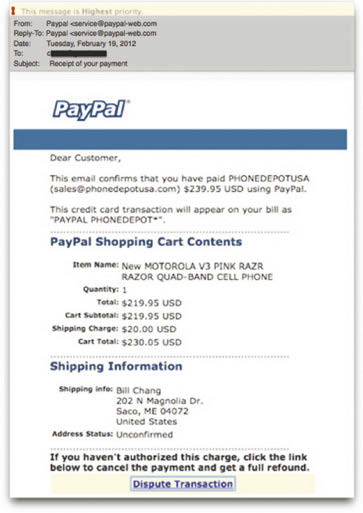
\includegraphics[width = 5cm]{figures/ChristopherHadn_2014_Kapitel2WasIstSocialE_SocialEngineeringEntt.jpg}
\caption{gefälschte E-Mail von PayPal}
\cite{GrundformenDesSE}
\label{fig:PhishingPayPal}
\end{figure}




\subsection{Elizitieren per Telefon}
\subsection{Identitätsbetrug}

\section{Zugangsarten}

\subsection{Elektronisch}
\subsection{Physischer}
\subsection{Soziale Medien}

\section{weitere Angriffsvektoren}

\subsection{Dumpster diving}
\subsection{Watering Hole}
\subsection{Ködern}
\subsection{Honigtopf}
\subsection{Tailgating/Piggybacking}
\subsection{Business Email Compromise}

\section{Psychologische Prinzipien hinter Social Engineering}

\subsection{Mittel der Manipulation}

\subsection{Mittel der Beeinflussung}

\subsubsection{stereotypes Verhalten}
\subsubsection{Reziprozität}
\subsubsection{Verpflichtung und Konsistenz}
\subsubsection{Soziale Bewährtheit}
\subsubsection{Sympathie}
\subsubsection{Authorität}
\subsubsection{Knappheit}

%\section{Beispiel eines erfolgreichen Social Engineering Angriffs}

\chapter{Social Engineering im Metaverse}\label{ch:SocialEngineeringimMV}

\section{Das Metaverse als Ziel für Social Engineering}

\subsection{Was macht das Metaverse interessant für Social Engineering}

\subsubsection{Charakterisierung der möglichen Zielpersonen}

\subsection{Gefahren für Minderjährige im Metaverse}

\section{Anwendungsmöglichkeiten von Social Engineering im Metaverse}

\subsubsection{Identitätsdiebstahl}
TODO

Beispiel Warframe

Im August 2022 wurde ich Zeuge, wie Social Engineering das Vertrauen seiner Opfer gezielt ausnutzt. Ein junges Mädchen, das neu im Spiel war, wurde von zwei erfahrenen Clan-Mitgliedern durch kleine Gefälligkeiten unterstützt. Sie schenkten ihr virtuelle Artefakte, die für neue Spieler sehr nützlich, für erfahrene Spieler jedoch wertlos sind. Zudem erklärten sie ihr, wie die verschiedenen Missionen im Spiel funktionieren und worauf sie achten muss.

Über ein halbes Jahr hinweg spielte das Mädchen regelmäßig mit den beiden und sammelte dabei eine Reihe wertvoller Ingame-Items. Da einige Aufgaben im Spiel zu schwierig für sie waren, boten die beiden Männer an, sich kurzzeitig in ihren Xbox-Account einzuloggen, um die schwierigen Missionen für sie zu erledigen. Sie wiesen sie sogar darauf hin, ein temporäres Passwort einzurichten, das sie nach erfolgreicher Mission wieder ändern könne. Durch Reziprozität und Sympathie beeinflusst, vertraute das Mädchen den Männern so sehr, dass sie schließlich ihre tatsächlichen Accountdaten weitergab, überzeugt davon, dass sie ihnen vertrauen konnte.

In ihrer Abwesenheit plünderten die Männer heimlich kleine Mnegen ihrer Ingame-Items und betrieben in ihrem Namen Handel. Zunächst bemerkte das Mädchen nichts davon. Erst während eines Urlaubs, als die Männer es übertrieben und auffällige Aktivitäten auf ihrem Account stattfanden, flog der Betrug auf. Die Accounts der Männer wurden daraufhin gesperrt, das Mädchen verzichtete jedoch auf eine Anzeige.


\subsection{Deep Fakes}
TODO

Avatar ist ein Gegenstand und kann lauschen
\subsection{Manipulation durch Gamification-Elemente}
\subsection{Biometrische Hacks}
TODO

Brillen können gehackt werden Biometrische Daten ausgelesen werden wie mimiken etc 

\subsection{blockchain Hacks}

Von Bedeutung ist dabei, dass es keine Kontrollinstanz gibt, die eingreifen kann, wenn der private Schlüssel verloren geht oder entwendet wird. Zudem bieten Wallet-Adressen allein keine ausreichende Identifikation der beteiligten Parteien.

\section{Auswirkungen des Social Engineering im Metaverse}

\subsection{persönliche Auswirkungen}
\subsection{soziale Auswirkungen}
\subsection{wirtschaftliche Auswirkungen}

\section{Fallbeispiel}

Fallstudie: Der Angriff auf VirtuCon
Hintergrund
VirtuCon war eine großangelegte virtuelle Konferenz im Metaverse, die auf einer populären Plattform für digitale Zusammenkünfte und Veranstaltungen stattfand. Die Konferenz zog Tausende von Teilnehmern an, darunter führende Experten in den Bereichen Technologie, Wirtschaft und Bildung. VirtuCon bot eine Vielzahl von Sitzungen, Workshops und Networking-Möglichkeiten in einer vollständig immersiven 3D-Umgebung.
Der Angriff
Einige Tage vor der Veranstaltung begannen die Organisatoren, Berichte über gefälschte Veranstaltungseinladungen zu erhalten, die an Teilnehmer gesendet wurden. Diese Einladungen enthielten Links, die angeblich zu exklusiven Vorregistrierungsboni oder speziellen Zugängen für die Konferenz führten. Tatsächlich leiteten diese Links die Nutzer jedoch auf gefälschte Login-Seiten, die darauf abzielten, persönliche Daten und Zugangsinformationen zu stehlen.
Parallel dazu schafften es die Angreifer, während der Veranstaltung mehrere Avatare zu kapern. Diese gekaperten Avatare wurden genutzt, um in verschiedenen Sitzungen und Chaträumen anwesend zu sein, wo sie weiterhin gefälschte Links verbreiteten und sogar versuchten, in private Gespräche einzudringen, um vertrauliche Informationen zu erlangen.
Analyse
Die Angreifer nutzten eine Kombination aus Phishing-Techniken und der Übernahme von Avataren, um das Vertrauen der Teilnehmer zu gewinnen und sie zur Preisgabe sensibler Informationen zu verleiten. Die Immersion und das Engagement im Metaverse trugen dazu bei, dass die Teilnehmer weniger misstrauisch gegenüber den ungewöhnlichen Aktivitäten waren, da sie die Interaktionen als Teil der Konferenzerfahrung ansahen.
Die psychologischen Tricks, die dabei zum Einsatz kamen, umfassten das Vorspiegeln von Dringlichkeit (durch das Angebot von "exklusiven Boni"), die Nutzung von Autorität und Vertrautheit (durch das Kapern bekannter Avatare) und das Ausnutzen der Neugier und des Wunsches nach Vernetzung der Teilnehmer.
Lessons Learned und Ableitungen für die Zukunft
Diese Fallstudie unterstreicht die Notwendigkeit umfassender Sicherheitsmaßnahmen und Awareness-Programme für Teilnehmer und Organisatoren von Veranstaltungen im Metaverse. Dazu gehören:
	• Verifizierung und Authentifizierung: Die Implementierung robuster Verifizierungs- und Authentifizierungsverfahren für alle Teilnehmer, Inhalte und Interaktionen.
	• Aufklärung und Training: Die Sensibilisierung der Nutzer für die Risiken und Anzeichen von Social Engineering-Angriffen.
	• Technische Sicherheitslösungen: Die Nutzung von Sicherheitstechnologien, um den Zugriff auf Veranstaltungen zu sichern und die Kommunikation zwischen Teilnehmern zu schützen.

\chapter{Schutzmechanismen und Abwehrstrategien}\label{ch:SchutzmechanismenundAbwehrstrategien}

\section{Technische Sicherheitsmaßnahmen}
\subsection*{copy}
• Verschlüsselung: Einsatz von Ende-zu-Ende-Verschlüsselung für Datenübertragungen innerhalb des Metaverse, um die Datensicherheit und Privatsphäre zu gewährleisten.\\
• Authentifizierung und Zugriffskontrolle: Verstärkung der Sicherheitsprotokolle durch Mehrfaktor-Authentifizierung und regelmäßige Überprüfung der Zugriffsrechte, um sicherzustellen, dass nur autorisierte Nutzer Zugang zu sensiblen Bereichen oder Informationen haben.\\
• Anomalieerkennung und Überwachung: Implementierung von Systemen zur Erkennung ungewöhnlicher Aktivitäten oder Verhaltensweisen, die auf einen Social Engineering-Angriff hindeuten könnten.\\

• Zwei-Faktor-Authentifizierung (2FA): Eine zusätzliche Sicherheitsebene für den Zugang zu virtuellen Umgebungen, die über das einfache Passwort hinausgeht.\\
• Ende-zu-Ende-Verschlüsselung: Sicherstellung, dass Kommunikation zwischen den Nutzern nicht von Dritten eingesehen werden kann.\\
• Regelmäßige Sicherheitsaudits: Überprüfung und Aktualisierung der Sicherheitseinstellungen und -protokolle, um Schwachstellen zu identifizieren und zu beheben.\\


\subsection*{eigene}


\section{Aufklärung und Bewusstseinsbildung}
TODO

Brillen können gehackt werden Biometrische Daten ausgelesen werden wie mimiken etc 

\section{Deep Fakes}
TODO

Avatar ist ein Gegenstand und kann lauschen
Technische Sicherheitsmaßnahmen

\chapter{Fazit und Ausblick}\label{ch:FazitundAusblick}

TODO

Sicherheit vorgegaukelt die so noch nicht vorhanden ist. Schwachstelle Mensch 
Ausblick auf zukünftige Entwicklungen und Forschungsbedarf



%\include{content/Zusammenfassung}


% remove if not needed
%\appendix
%\include{content/a1_supplemental}

\backmatter
%Tabellenverzeichnis
%\listoftables
\cleardoublepage

%\renewcommand{\lstlistlistingname}{List of Listings}  % change for German thesis
%\lstlistoflistings
%\cleardoublepage

\bibliographystyle{wmaainf}
\bibliography{refs}

\listoffigures
\cleardoublepage

\printnoidxglossaries

\end{document}
